\section{Methodology}
\label{sec:tist_methodology}

Consider a labeled source dataset, $\mathcal{S}$, with training images $\mathcal{X_S}$ and corresponding segmentation labels $\mathcal{Y_S}$, while we denote a target dataset $\mathcal{T}$, containing only target images $\mathcal{X_T}$. We aim to train a network using $\mathcal{X_S}$, $\mathcal{Y_S}$, and $\mathcal{X_T}$ for semantic segmentation in the target dataset. 


We propose to train the model using a self-supervised approach on the images $\mathcal{X_T}$ by assigning pseudo labels during training. Typical pseudo labels are computed from independent predictions of unlabeled images. Instead, our proposed framework adopts a self-assessment strategy to determine the reliability of predictions in an unsupervised fashion. Specifically, we propose to target highly-reliable predictions generated by a network aiming for transformation-invariant confidence. Compared to self-ensembling strategies that penalize the distant predictions corresponding to the transformed versions of identical inputs, our goal is to filter out transformation-variant predictions. Indeed, our method reinforces the ensemble of high-confidence predictions from two versions of the same target sample. Our proposed TI-ST framework simultaneously trains on the source and target domains, so as to progressively bridge the intra-domain distribution gap. \cref{fig:BD} depicts our TI-ST framework, which we detail in the following sections. 

%\begin{figure}[t]
%\centering
%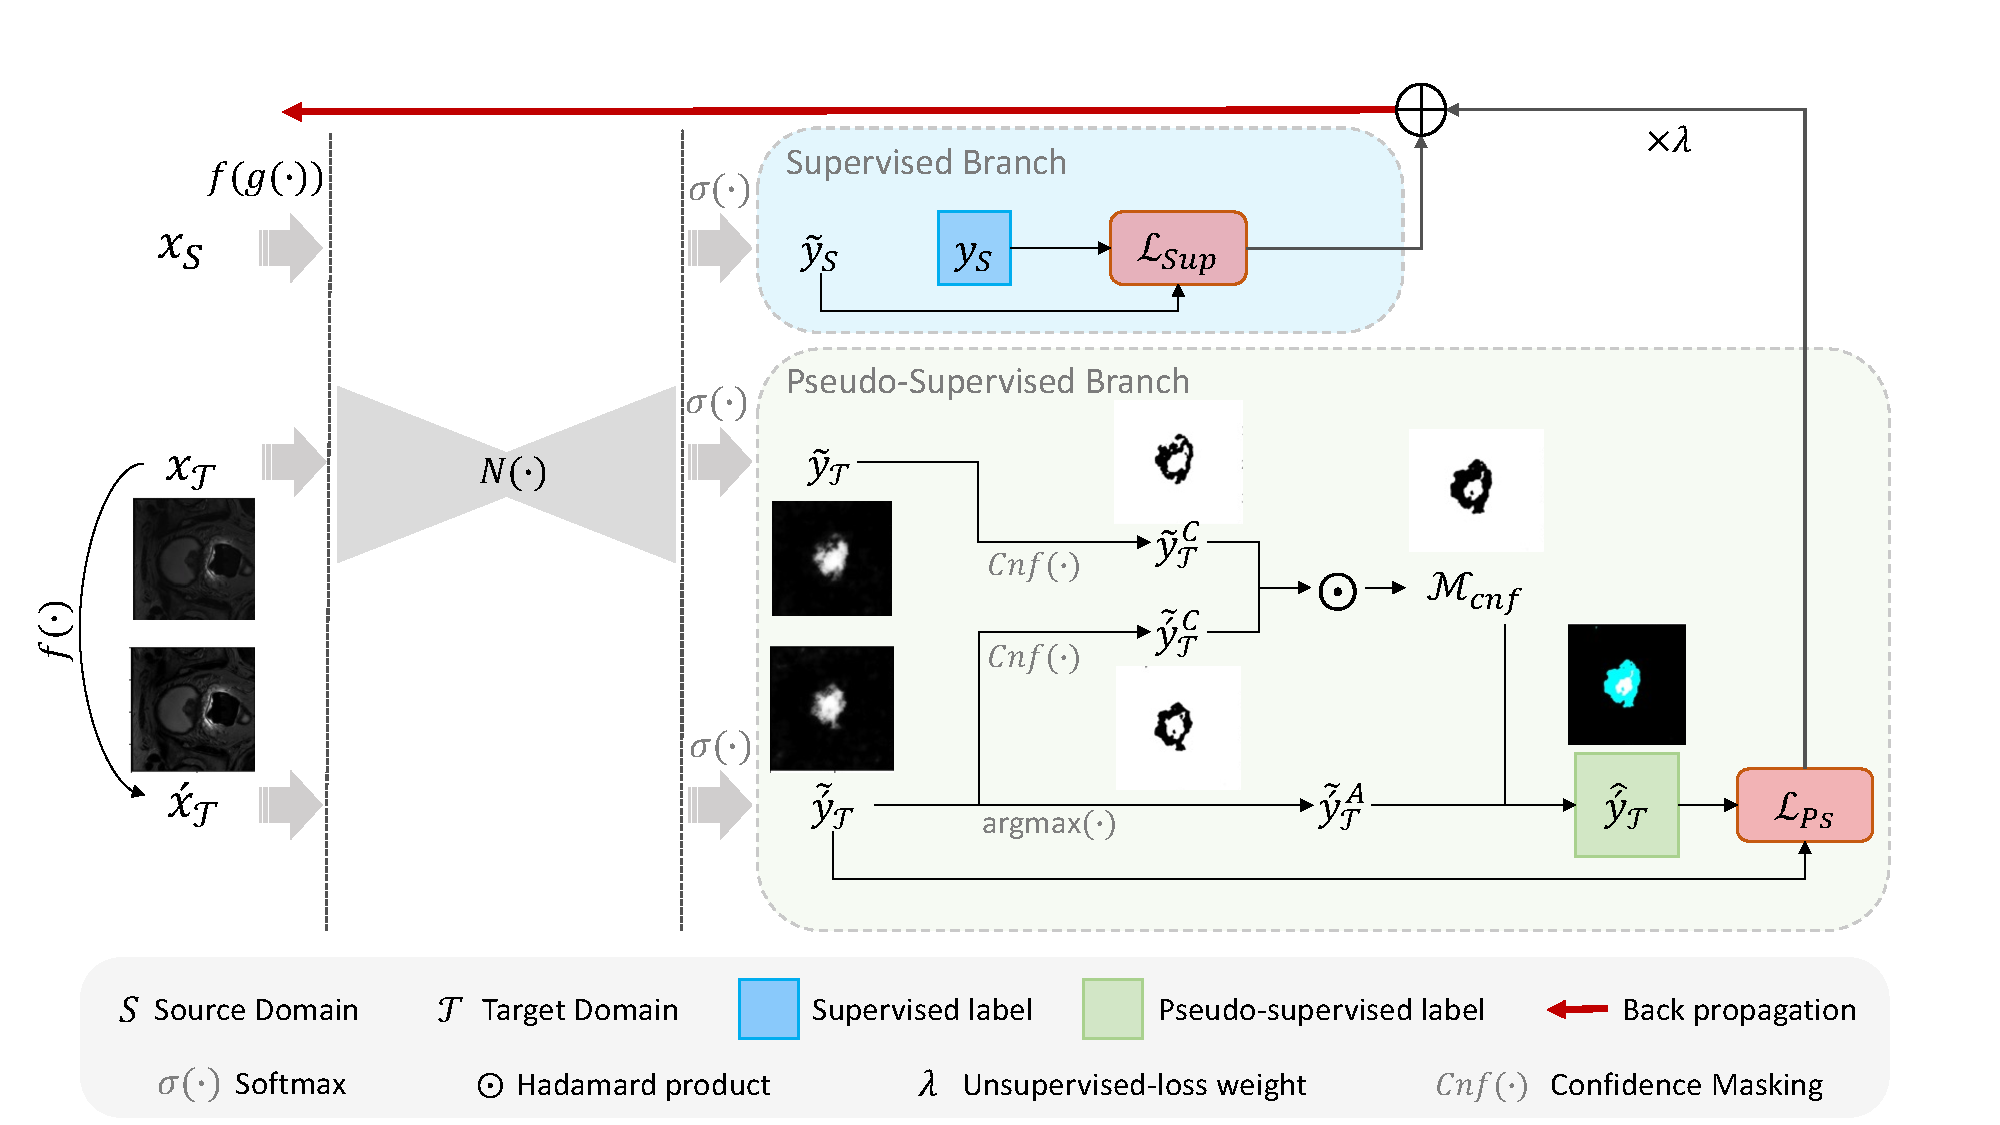
\includegraphics[width=\textwidth]{figures/BD8.pdf}
%\caption{Proposed unsupervised domain adaptation framework based on transformation-invariant self-training (TI-ST). Ignored pseudo-labels during unsupervised loss computation are shown in turquoise.
%}
%\label{fig:BD}
%\end{figure}

\plainwidefig{1}{figures/BD8.pdf}{Proposed unsupervised domain adaptation framework based on transformation-invariant self-training (TI-ST). Ignored pseudo-labels during unsupervised loss computation are shown in turquoise.}{fig:BD}

\subsection{Model} At training time, images from the source dataset are augmented using spatial $g(\cdot)$ and non-spatial $f(\cdot)$ transformations and passed through a segmentation network, $N(\cdot)$, by which the network is trained using a standard supervision loss. At the same time, images from the target dataset are also passed to the network. Specifically, we feed two versions of each target image to the network: (1) the original target image $x_\mathcal{T}$, and (2) its non-spatially transformed version, $\Acute{x_\mathcal{T}} = f(x_\mathcal{T})$. 
% \RS{There is no other mention of $f$ throughout the method. We should probably give some information as to what we use, and why.} 
Once fed through the network, the corresponding predictions can be defined as $\tilde{y_{\mathcal{T}}} = \sigma(N(x_{\mathcal{T}}))$ and $\tilde{\acute{y_{\mathcal{T}}}} = \sigma(N(\Acute{x_{\mathcal{T}}}))$, where $\sigma(\cdot)$ is the Softmax operation. We then define a confidence-mask ensemble as
\begin{equation}
\mathcal{M}_{cnf} = 
Cnf(\tilde{{y_{\mathcal{T}}}})
\odot
Cnf(\tilde{\Acute{y_{\mathcal{T}}}}),
\label{eq: ensemble of confidence}
\end{equation}
\noindent
where $\odot$ refers to Hadamard product used for element-wise multiplication, and $Cnf$ is the high confidence masking function,
\iffalse
\begin{equation}
    \mathcal{M}_{cnf}(\tilde{\acute{y_T}}, \Acute{\tilde{y_T}}) = h(\tilde{\acute{y_T}})\odot h(\Acute{\tilde{y_T}})
    \label{eq: confidence mask}
\end{equation}
\fi
\begin{equation}
    Cnf_{\textsub{$\in (W\times H$)}}(y) =
    \begin{cases}
    0, & \text{if    } \maxH_{\textsub{C}}(y) > \uptau\\
    1, & \text{else.  }
    \end{cases}
    \label{eq: filtering}
\end{equation}
\noindent
where $\uptau \in (0.5,1) $ is the confidence threshold, and $H$, $W$, and $C$ are the height, width, and number of classes in the output, respectively. Specifically, $\mathcal{M}_{cnf}$ encodes regions of confident predictions that are invariant to transformations.
We can then compute the pseudo-ground-truth mask for each input from the target dataset as
\begin{equation}
\hat{\Acute{y_{\mathcal{T}}}} = 
\begin{cases}
\argmaxH_{\textsub{C}} (\tilde{\Acute{y_{\mathcal{T}}}}), & \text{if  } \:\mathcal{M}_{cnf} = 1\\
\text{ignore}, & \text{else.  }
\end{cases}
\end{equation}
\noindent

\subsection{Training}
To train our model, we simultaneously consider both the source and target samples by minimizing the following loss,
\begin{equation}
    \mathcal{L}_{overall} = \mathcal{L}_{Sup}( \tilde{y_\mathcal{S}}, y_\mathcal{S}) + \lambda \Big(\mathcal{L}_{Ps}(\mu (\tilde{\Acute{y_{\mathcal{T}}}}), \hat{\Acute{y_{\mathcal{T}}}})\Big) ,
    \label{eq: loss}
\end{equation}
\noindent
where $\mathcal{L}_{Sup}$ and $\mathcal{L}_{Ps}$ indicate the supervised and pseudo-supervised loss functions used, respectively. We set $\lambda$ as a time-dependent weighing function that gradually increases the share of pseudo-supervised loss. Intuitively, our pseudo-supervised loss enforces predictions on transformation-invariant highly-confident regions for unlabeled images. 

\subsubsection{Discussion} 
The quantity and distribution of supervised data are determining factors in neural networks' performance. With highly distributed large-scale supervisory data, neural networks converge to an optimal state efficiently. However, when only limited supervisory data, with heterogeneous distribution from the inference dataset, using more sophisticated methods to leverage a priori knowledge is essential. Our proposed use of invariance of network predictions with respect to data augmentation is a strong form of knowledge that can be learned through dataset-dependent augmentations. The trained network is then expected to provide consistent predictions under diverse transformations. Hence, the transformation variance of the network predictions can indicate the network's prediction doubt and low confidence correspondingly. We take advantage of this characteristic to assess the reliability of predictions and filter out unreliable pseudo-labels.
